\section{Durchführung}
\label{sec:Durchführung}
Der Versuch ist wie in Abbildung \ref{pic:aufbau} aufgebaut.
\begin{figure}
    \centering
    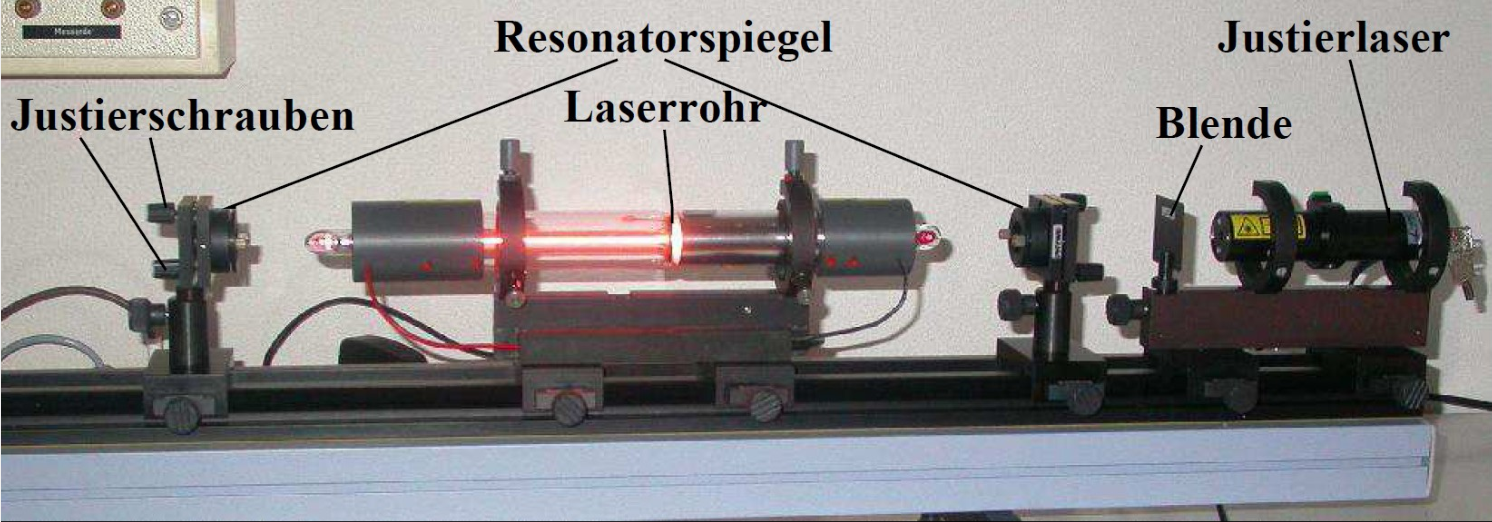
\includegraphics[width = 0.78\textwidth]{pics/Laseraufbau.png}
    \caption{Versuchsaufbau des He-Ne-Lasers.\cite{V61}}
    \label{pic:aufbau}
\end{figure}
Dabei befinden sich ein Justierlaser, eine Blende, die Laserröhre und die beiden Spiegel auf einer
optischen Schiene. Das Laserrohr hat eine Länge von $l = \SI{408}{\milli\meter}$ und einen Durchmesser von $d = \SI{1.1}{\milli\meter}$.
Der Justierlaser ist vorjustiert und kann zur Justage
des HeNe-Lasers genutzt werden. Dafür werden die reflektierten Strahlen des Lasers, durch drehen und justieren der Spiegel,
auf der Blende mit dem Ursprungsstrahl überlagert. Sind alle drei Strahlen aufeinander ist der Laser vorjustiert.
Folgend wird der Strom der Hochspannung auf $\SI{6.5}{\milli\ampere}$ gestellt und eine
Feinjustage vollzogen bis die Lasertätigkeit einsetzt.

\subsection{Überprüfen der Stabilitätsbedingung}
Die Stabilitätsbedingung wird überprüft, indem der maximale Resonatorabstand
für verschiedene Linsen vermessen wird.
Dazu wird zuerst ein planarer und ein konkaver Spiegel ($r = \SI{1400}{\milli\meter\per flat}$) verwendet.
Die Resonatorlänge wird mit Hilfe einer Photodiode hinter dem teildurchlässigen Spiegel auf den minimalen Wert und auf die maximale Leistung eingestellt.
In $\SI{10}{\centi\meter}$-Schritten wird nun die Resonatorlänge erhöht bis keine Lasertätigkeit mehr möglich ist.
Dann wird der planare Spiegel durch einen weiteren konkaven Spiegel ($r = \SI{1400}{\milli\meter\per flat}$)
ersetzt und die Resonatorlänge in $\SI{20}{\centi\meter}$-Schritten bis zur maximalen Länge erhöht.
Dabei wird nach jedem Schritt die Leistung des Lasers maximiert.
In der Nähe des maximalen Werts werden in beiden Messreihen kleinere Abstände eingestellt um möglichst genau die 
Stabilität zu bestimmen.

\subsection{Untersuchung der TEM-Moden}
In den folgenden Versuchsteilen wird nur der Resonator aus zwei konkaven Spiegeln verwendet.
Mithilfe eines Golddrahtes ($d = \SI{0.005}{\milli\meter}$), welcher zwischen Spiegel und Laserrohr verbaut ist,
werden verschiedene Moden stabilisiert. Diese werden an einem optischen Schirm mithilfe einer Streulinse vergrößert.
Daraufhin wird mit einer Photodiode die Strahlintensität der $\symup{TEM_{00}}$-Mode und der $\symup{TEM_{10}}$-Mode in abhängigkeit der Position aufgenommen.

\subsection{Bestimmung der Polarisation}
Eine Resonatorlänge von $L = \SI{143}{\centi\meter}$ wird eingestellt.
Die Polarisation wird mit Hilfe eines hinter dem Auskoppelspiegel angebrachtem Polarisators vermessen. 
Dazu wird der Polarisator in $\ang{10}$-Schritten gedreht und die Strahlintensität mit einer Photodiode vermessen.

\subsection{Longitudinale Moden}
Um die Schwebungsfrequenzen zu messen wird eine schnelle Photodiode hinter dem Auskopplungsspiegel plaziert.
Die Photodiode wird mit dem Spektrumanalysator verbunden.
Danach wird für fünf verschiedene Resonatorlängen ein Frequenzspektrum aufgenommen.

\subsection{Bestimmung der Wellenlänge}
Der Resonator wird auf eine Länge von $L = \SI{143}{\centi\meter}$ eingestellt.
Zudem werden vier Gitter mit Gitterkonstanten von $g = \SI{80}{\per\milli\meter}$, 
$g = \SI{100}{\per\milli\meter}$, $g = \SI{600}{\per\milli\meter}$ und $g = \SI{1200}{\per\milli\meter}$
nacheinander hinter den Auskopplungsspiegel plaziert. 
Die Breite der auf dem Schirm sichtbaren Maxima wird daraufhin vermessen.
